\documentclass[border=12pt]{standalone}
\usepackage[table,dvipsnames]{xcolor}
\usepackage{tikz}
\usetikzlibrary{arrows.meta,positioning,fit,backgrounds}
\usepackage{array}

% ---- colors ----
\definecolor{schemagreen}{RGB}{198,239,206}
\definecolor{domsub}{RGB}{255,224,178}
\definecolor{ransub}{RGB}{197,233,243}
\definecolor{hdr}{RGB}{225,225,225}
\definecolor{agentfill}{RGB}{231,222,242}
\definecolor{midfill}{RGB}{218,232,247}
\definecolor{leaffill}{RGB}{244,248,253}
\definecolor{darknavy}{RGB}{18,32,86}

\begin{document}
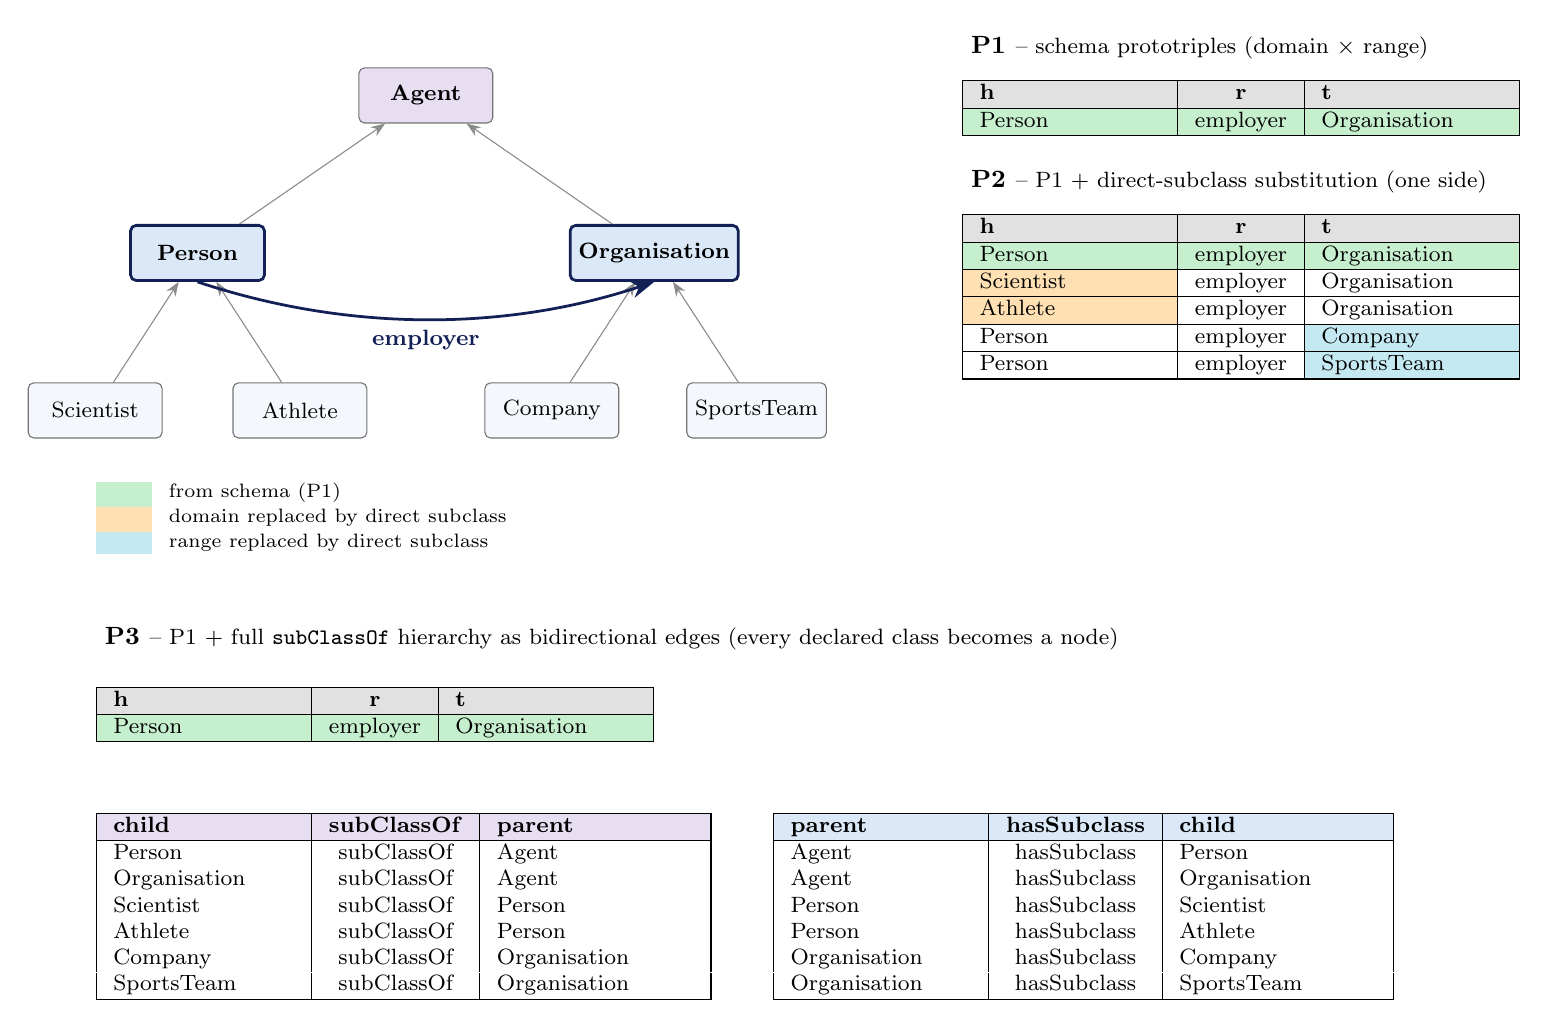
\begin{tikzpicture}[
  font=\footnotesize,
  cls/.style={draw=black!55, rounded corners=2pt, minimum height=7mm,
              minimum width=17mm, inner sep=3pt, fill=leaffill},
  root/.style={cls, fill=agentfill, font=\footnotesize\bfseries},
  ep/.style={cls, fill=midfill, draw=darknavy, line width=1pt, font=\footnotesize\bfseries},
  sub/.style={-{Stealth[length=1.8mm]}, draw=black!45},
  tbl/.style={anchor=north west, inner sep=0pt},
]

% ===================== LEFT: class hierarchy (no owl:Thing) =====================
\node[root] (agent) at (4.2,4) {Agent};

\node[ep] (person) at (1.3,2) {Person};
\node[ep] (org)    at (7.1,2) {Organisation};

\node[cls] (sci)    at (0,0)   {Scientist};
\node[cls] (ath)    at (2.6,0) {Athlete};
\node[cls] (comp)   at (5.8,0) {Company};
\node[cls] (team)   at (8.4,0) {SportsTeam};

% subClassOf edges (child -> parent)
\draw[sub] (person) -- (agent);
\draw[sub] (org)    -- (agent);
\draw[sub] (sci)    -- (person);
\draw[sub] (ath)    -- (person);
\draw[sub] (comp)   -- (org);
\draw[sub] (team)   -- (org);

% employer relation: domain Person -> range Organisation
\draw[-{Stealth[length=3mm]}, line width=1pt, darknavy]
  (person.south) .. controls (3.2,1.0) and (5.2,1.0) .. (org.south)
  node[pos=0.5, below=0pt, font=\footnotesize\bfseries] {employer};

% legend (left, under the hierarchy -- clear of the P3 block)
\node[tbl, font=\scriptsize] at (0,-0.9) {%
\begin{tabular}{ll}
\cellcolor{schemagreen}\phantom{xx} & from schema (P1)\\[1pt]
\cellcolor{domsub}\phantom{xx} & domain replaced by direct subclass\\[1pt]
\cellcolor{ransub}\phantom{xx} & range replaced by direct subclass\\
\end{tabular}};

% ===================== RIGHT: P1 and P2 =====================
\node[anchor=west, font=\small\bfseries] at (11,4.6) {P1 \footnotesize\mdseries -- schema prototriples (domain $\times$ range)};
\node[tbl] at (11,4.2) {%
\begin{tabular}{|>{\raggedright\arraybackslash}p{23mm}|c|>{\raggedright\arraybackslash}p{23mm}|}
\hline
\rowcolor{hdr}\textbf{h}&\textbf{r}&\textbf{t}\\\hline
\rowcolor{schemagreen}Person & employer & Organisation\\\hline
\end{tabular}};

\node[anchor=west, font=\small\bfseries] at (11,2.9) {P2 \footnotesize\mdseries -- P1 $+$ direct-subclass substitution (one side)};
\node[tbl] at (11,2.5) {%
\begin{tabular}{|>{\raggedright\arraybackslash}p{23mm}|c|>{\raggedright\arraybackslash}p{23mm}|}
\hline
\rowcolor{hdr}\textbf{h}&\textbf{r}&\textbf{t}\\\hline
\rowcolor{schemagreen}Person & employer & Organisation\\\hline
\cellcolor{domsub}Scientist & employer & Organisation\\\hline
\cellcolor{domsub}Athlete   & employer & Organisation\\\hline
Person & employer & \cellcolor{ransub}Company\\\hline
Person & employer & \cellcolor{ransub}SportsTeam\\\hline
\end{tabular}};

% ===================== BOTTOM: P3 =====================
\node[anchor=west, font=\small\bfseries] at (0,-2.9)
  {P3 \footnotesize\mdseries -- P1 $+$ full \texttt{subClassOf} hierarchy as bidirectional edges (every declared class becomes a node)};

\node[tbl] at (0,-3.5) {%
\begin{tabular}{|>{\raggedright\arraybackslash}p{23mm}|c|>{\raggedright\arraybackslash}p{23mm}|}
\hline
\rowcolor{hdr}\textbf{h}&\textbf{r}&\textbf{t}\\\hline
\rowcolor{schemagreen}Person & employer & Organisation\\\hline
\end{tabular}};

\node[tbl] at (0,-5.1) {%
\begin{tabular}{|>{\raggedright\arraybackslash}p{23mm}|c|>{\raggedright\arraybackslash}p{25mm}|}
\hline
\rowcolor{agentfill}\textbf{child}&\textbf{subClassOf}&\textbf{parent}\\\hline
Person       & subClassOf & Agent\\
Organisation & subClassOf & Agent\\
Scientist    & subClassOf & Person\\
Athlete      & subClassOf & Person\\
Company      & subClassOf & Organisation\\
SportsTeam   & subClassOf & Organisation\\\hline
\end{tabular}};

\node[tbl] at (8.6,-5.1) {%
\begin{tabular}{|>{\raggedright\arraybackslash}p{23mm}|c|>{\raggedright\arraybackslash}p{25mm}|}
\hline
\rowcolor{midfill}\textbf{parent}&\textbf{hasSubclass}&\textbf{child}\\\hline
Agent        & hasSubclass & Person\\
Agent        & hasSubclass & Organisation\\
Person       & hasSubclass & Scientist\\
Person       & hasSubclass & Athlete\\
Organisation & hasSubclass & Company\\
Organisation & hasSubclass & SportsTeam\\\hline
\end{tabular}};

\end{tikzpicture}
\end{document}
